\documentclass{book}
\usepackage{ardour,graphicx}
\title{Ardour 3 --- A users' manual}
\author{The Ardour Community}
\date{}
\begin{document}

\maketitle

\tableofcontents

\chapter{Introduction}

Hello, and welcome to Ardour!

\section{What is Ardour?}

Ardour is an open-source digital audio workstation (DAW) for Linux and Mac OS~X.


\section{Typographical conventions}

This manual takes a cue from the \TeX{}book and uses special symbols
to denote sections which contain advanced material.  Readers can
skip these sections without any great loss.

\begin{danger}
Tricky parts of the text are marked with a `bend in the road' marker.
They contain extra information which may be of interest to advanced
users.
\end{danger}

\begin{ddanger}
Especially tricky parts of the text are marked with a double
bend-in-the-road marker.  Such sections will only be of interest to
the completist or serious hacker.
\end{ddanger}


\chapter{Overview}

As one might expect, Ardour is similar in many ways to many other DAWs
and also has its fair share of differences.  This chapter gives an
overview of Ardour.


\section{JACK}

Ardour is built on another piece of software called JACK\footnote{JACK
  stands for the JACK Audio Connection Kit; a pleasingly recursive acronym}.
JACK has two main functions; first, it moves audio and MIDI to
and from your sound card, and second, it allows audio and MIDI to be
routed between different applications.

JACK provides a great deal of flexibility and power, especially when
running other applications (such as soft-synthesizers or samplers) at
the same time as Ardour.  It is somewhat similar to Steinberg's Rewire
technology, though broader in scope.  It is even possible to use JACK
to route audio and MIDI over network connections.

JACK is so important to Ardour's operation that it earns its own
discussion in chapter~\ref{ch:jack}.


\section{Sessions}

An Ardour \emph{session} is a container for an entire project.  A
session may contain an arbitrary number of tracks and busses
consisting of audio and MIDI data, along with information on processing
those tracks, a mix of levels, and everything else related to the
project.  A session might typically contain a song, or perhaps an entire
album or a complete live recording.

Ardour sessions are held in directories; these directories contain one
or more \emph{session files}, some or all of the audio and MIDI data
and a number of other state files that Ardour requires.  The session
file describes the structure of the session, and holds automation data
and other details.

\begin{danger}
Ardour's session file is kept in XML format, which is advantageous as
it is somewhat human-readable, and human-editable in a crisis!  Sound
files are stored in one of a number of optional formats, and MIDI
files as SMF (standard MIDI format).

It is also possible for Ardour sessions to reference sound and MIDI
files outside the session directory.
\end{danger}

Ardour has a current session at all times; if you load Ardour without
specifying one, it will offer to load or create one for you.



\section{Tracks}

A track is a concept common to most DAWs, and used also in Ardour.
Tracks can record audio or MIDI data to disk, and then replay it with
processing.  They also allow the audio or MIDI data to be edited in a
variety of different ways.

In a typical pop production, one might use a track each for the kick
drum, another for the snare, more perhaps for the drum overheads and
others for bass, guitars and vocals.

Ardour can record to any number of tracks at one time, and then play
those tracks back.  On playback, a track's recordings may be processed
by any number of plugins, panned, and its level altered to achieve a
suitable mix.

\begin{danger}
A track's type is really only related to the type of data that it
stores on disk.  It is possible, for example, to have a MIDI track
with a synthesizer plugin which converts MIDI to audio.  Even though
the track remains `MIDI', in the sense that its on-disk recordings are
MIDI, its output may be audio-only.
\end{danger}


\section{Regions}

A track may contain many segments of audio or MIDI\@.  Ardour contains
these segments in things called \emph{regions}, which are
self-contained snippets of audio or MIDI data.  Any recording pass,
for example, generates a region on each track that is enabled for
recording.  Regions can be subjected to many editing operations; they
may be moved around, split, trimmed, copied, and so on.


\section{Playlists}

The details of what exactly each track should play back is described
by a \emph{playlist}.  A playlist is simply a list of regions; each
track always has an active playlist, and a track's current playlist
can always be changed.


\section{Busses}

Busses are another common concept in both DAWs and hardware mixers.
They are similar in many ways to tracks; they process audio or MIDI,
and can run processing plugins.  The only difference is that their
input is obtained from other tracks or busses, rather than from disk.

One might typically use a buss to collect together the outputs of
related tracks.  Consider, for example, a 3-track recording of a
drum-kit; given kick, snare and overhead tracks, it may be helpful to
connect the output of each to a bus called `drums', so that the
drum-kit's level can be set as a unit, and processing (such as
equalisation or compression) can be applied to the mix of all tracks.


\chapter{JACK}
\label{ch:jack}

\chapter{Quick start}

This chapter blithely assumes that the reader just wants to use Ardour
to make a basic recording, and describes how that can be achieved.

\section{Starting Ardour and creating a session}

\begin{figure}[ht]
\begin{center}
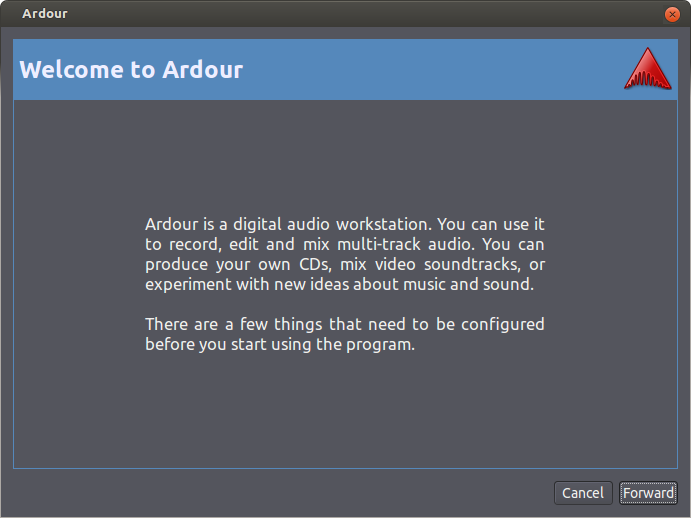
\includegraphics[scale=0.5]{screenshots/welcome-to-ardour.png}
\end{center}
\caption{Welcome to Ardour!}
\label{fig:welcome-to-ardour}
\end{figure}

\begin{figure}[ht]
\begin{center}
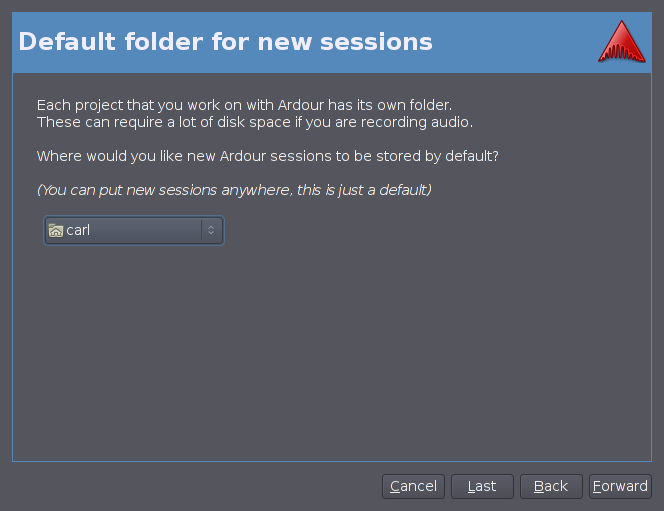
\includegraphics[scale=0.5]{screenshots/default-folder-for-new-sessions.png}
\end{center}
\caption{Default folder for new sessions}
\label{fig:default-folder-for-new-sessions}
\end{figure}

\begin{figure}[ht]
\begin{center}
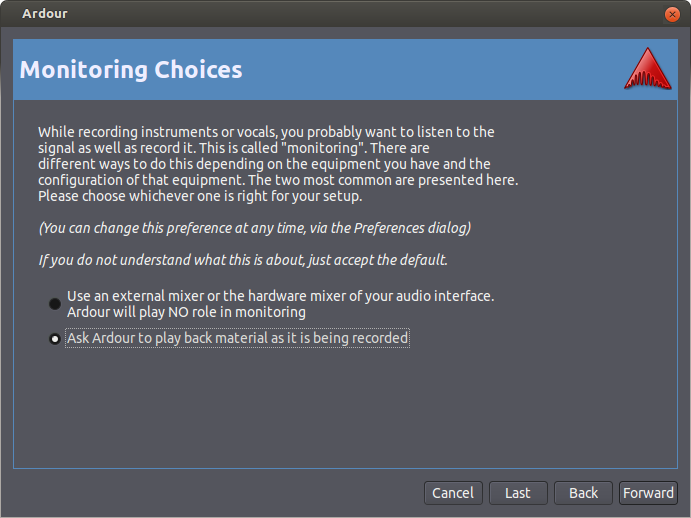
\includegraphics[scale=0.5]{screenshots/monitoring-choices.png}
\end{center}
\caption{Monitoring choices}
\label{fig:monitoring-choices}
\end{figure}

\begin{figure}[ht]
\begin{center}
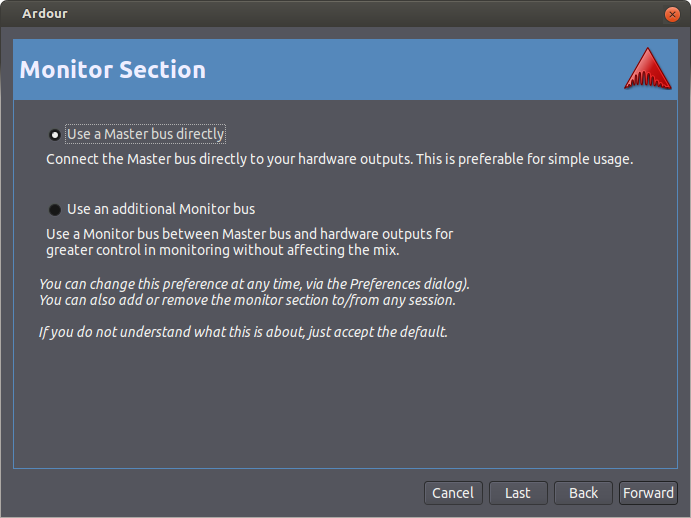
\includegraphics[scale=0.5]{screenshots/monitor-section.png}
\end{center}
\caption{Monitor section}
\label{fig:monitor-section}
\end{figure}

\begin{figure}[ht]
\begin{center}
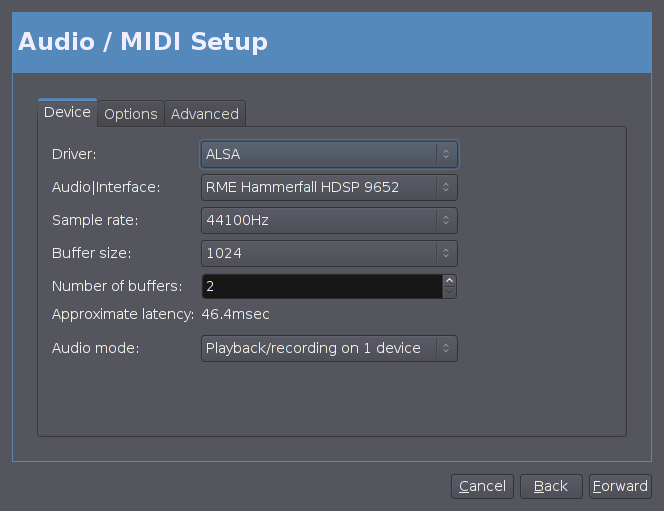
\includegraphics[scale=0.5]{screenshots/audio-midi-setup-device.png}
\end{center}
\caption{Audio/MIDI setup --- device}
\label{fig:audio-midi-setup-device}
\end{figure}

\begin{figure}[ht]
\begin{center}
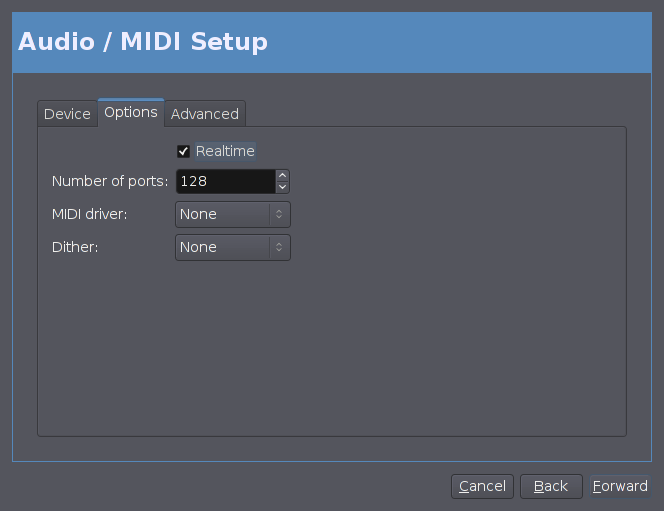
\includegraphics[scale=0.5]{screenshots/audio-midi-setup-options.png}
\end{center}
\caption{Audio/MIDI setup --- options}
\label{fig:audio-midi-setup-options}
\end{figure}

\begin{figure}[ht]
\begin{center}
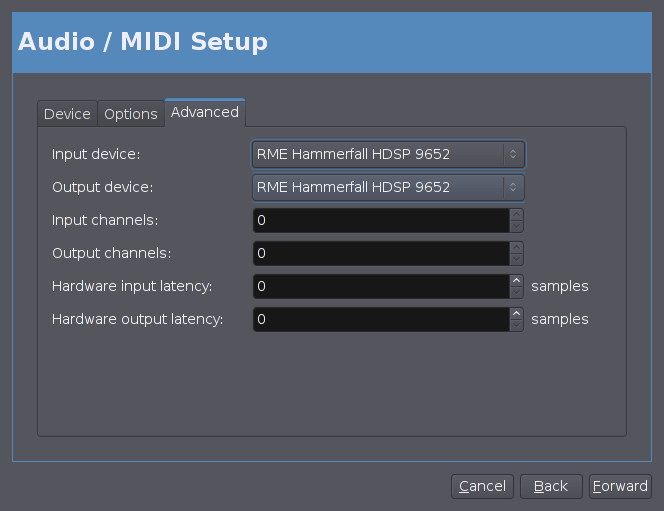
\includegraphics[scale=0.5]{screenshots/audio-midi-setup-advanced.png}
\end{center}
\caption{Audio/MIDI setup --- advanced}
\label{fig:audio-midi-setup-advanced}
\end{figure}

\begin{figure}[ht]
\begin{center}
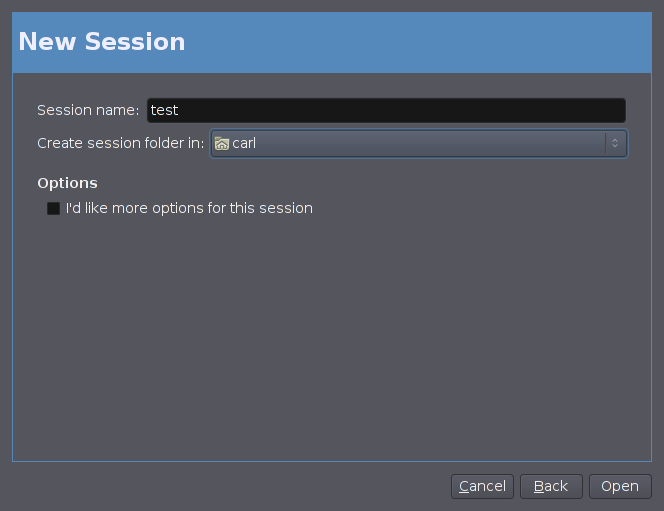
\includegraphics[scale=0.5]{screenshots/new-session.png}
\end{center}
\caption{New session}
\label{fig:new-session}
\end{figure}

\begin{figure}[ht]
\begin{center}
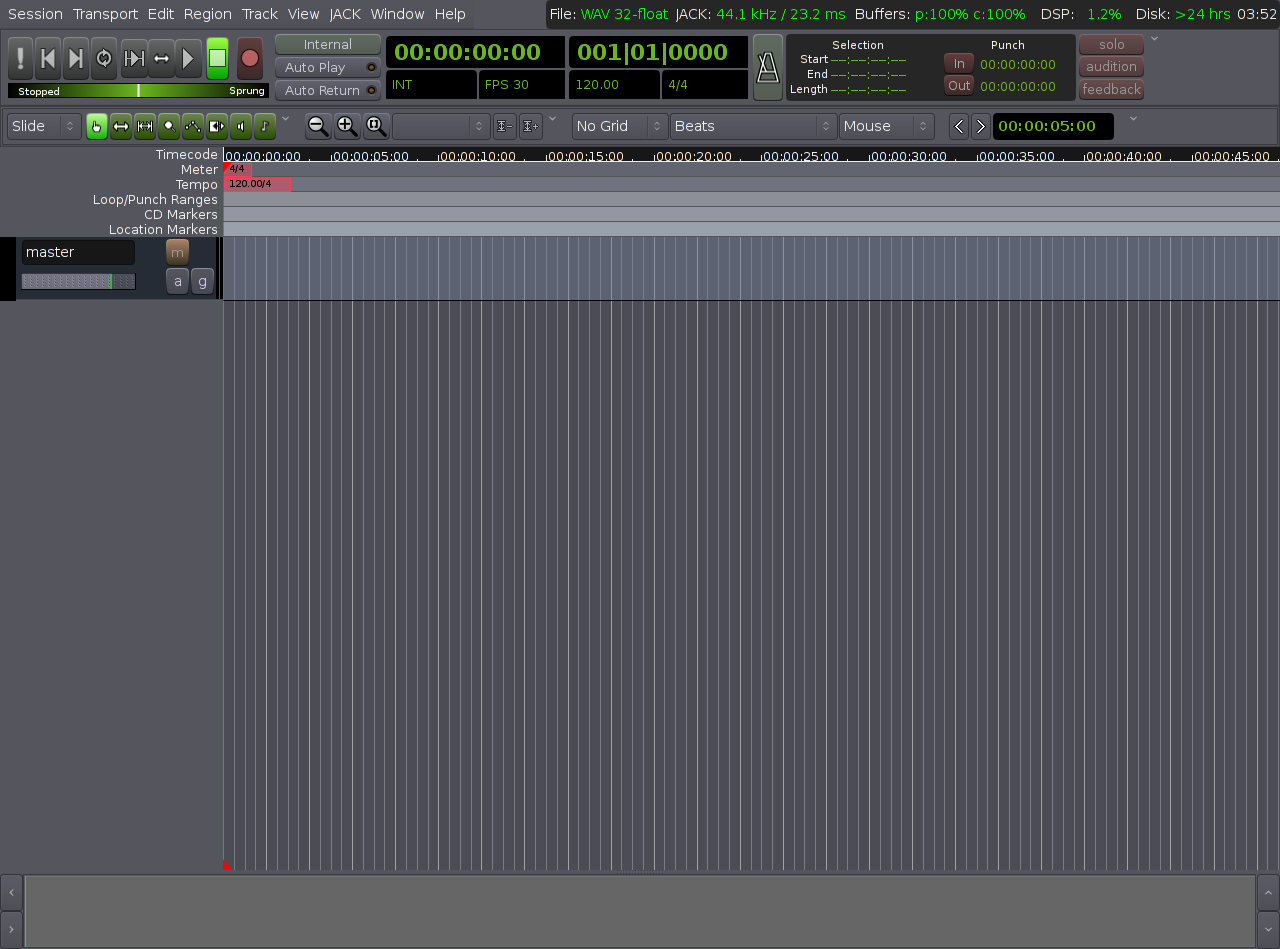
\includegraphics[scale=0.3]{screenshots/editor.png}
\end{center}
\caption{\ldots and finally: the editor!}
\label{fig:editor}
\end{figure}

\section{Adding a track and connecting it up}

\section{Recording}

\section{Adding another track as an overdub}

\section{Mix-down}

\section{Export}



\end{document}



